\documentclass[tikz,border=6pt]{standalone}
\usepackage{xcolor}
\begin{document}
% Canonical ch-diagram for 2_1^1
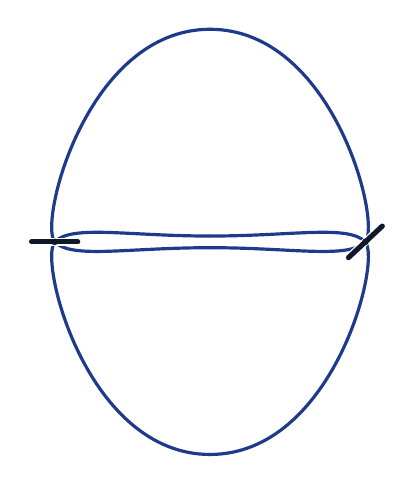
\begin{tikzpicture}[line join=round]
  \definecolor{skcomp0}{RGB}{30,58,138}
  \definecolor{skmark}{RGB}{15,23,42}
  \draw[skcomp0, line width=1.15pt, line cap=round] (-1.9339,-0.0000) .. controls (-2.1386,0.2589) and (-1.5195,2.7000) .. (0.0393,2.7000);
  \draw[skcomp0, line width=1.15pt, line cap=round] (2.0125,-0.0000) .. controls (2.2172,0.2589) and (1.5982,2.7000) .. (0.0393,2.7000);
  \draw[skcomp0, line width=1.15pt, line cap=round] (-1.9339,-0.0000) .. controls (-2.1386,-0.2589) and (-1.5195,-2.7000) .. (0.0393,-2.7000);
  \draw[skcomp0, line width=1.15pt, line cap=round] (2.0125,-0.0000) .. controls (2.2172,-0.2589) and (1.5982,-2.7000) .. (0.0393,-2.7000);
  \draw[skcomp0, line width=1.15pt, line cap=round] (-1.9339,-0.0000) .. controls (-1.7135,-0.2204) and (-1.0201,-0.0740) .. (0.0393,-0.0740);
  \draw[skcomp0, line width=1.15pt, line cap=round] (2.0125,-0.0000) .. controls (1.7921,-0.2204) and (1.0987,-0.0740) .. (0.0393,-0.0740);
  \draw[skcomp0, line width=1.15pt, line cap=round] (-1.9339,-0.0000) .. controls (-1.7135,0.2204) and (-1.0201,0.0740) .. (0.0393,0.0740);
  \draw[skcomp0, line width=1.15pt, line cap=round] (2.0125,-0.0000) .. controls (1.7921,0.2204) and (1.0987,0.0740) .. (0.0393,0.0740);
  \draw[white, line width=2.8pt, line cap=round] (-2.2273,-0.0000) -- (-1.6405,-0.0000);
  \draw[skmark, line width=1.85pt, line cap=round] (-2.2273,-0.0000) -- (-1.6405,-0.0000);
  \fill[skmark] (-1.9339,-0.0000) circle (1.2pt);
  \draw[white, line width=2.8pt, line cap=round] (2.2273,0.1999) -- (1.7978,-0.1999);
  \draw[skmark, line width=1.85pt, line cap=round] (2.2273,0.1999) -- (1.7978,-0.1999);
  \fill[skmark] (2.0125,-0.0000) circle (1.2pt);
\end{tikzpicture}
\end{document}
